\chapter{Introduction}
\label{ch:intro}
% need to open with a 


As researchers first started to build technology to help us communicate with other people at a distance, a consensus on what our systems should aspire to do quickly arose: computer mediated communication systems should focus on recreating the experience of being face-to-face with another person. The best system, in this model, is one that seems to disappear in the same way that the best window makes us feel like there is nothing between us and what is on the other side of the glass. Since the early 1970s, it has seemed like we have always been on the verge of a utopian environment where distance disappears and we interact as richly with friends, family, and colleagues around the world as we do with someone sitting in the same room. \citep{Egido:1988vq} And yet, like the paperless office \citep{Sellen:2001uk}, this future has failed to materialize. We can interpret this in two ways: either our tools have failed to deliver on the promise of a ``being there'' level experience or our persistent selection of non-``being there'' experiences reveals a broad desire for a different vision of computer mediated communication. As with \citet{Hollan:1992tz}, I will argue the latter case. In particular, I will focus on how  computer-mediated-communication tools can complement existing interaction contexts. I will show through a series of design projects and studies where we might find ways to create experiences that meet the challenge of being ``beyond being there''; experiences that are compelling precisely because they are trying to be something other than just a face-to-face presence with others.

To introduce this design space, I describe the broader context of computer-mediated-communication systems and why work has long focused on the ``being there'' approach to design. I will discuss approaches described in the literature for thinking about the different design strategies one might employ when trying to build new systems with a ``beyond being there'' approach in mind.

% My research has focused on designing, building, deploying, and observing the use of computer mediated communication systems that complement existing communication technologies and face-to-face interaction. In this dissertation, I will introduce a new theoretical framework for thinking about this category of design and trace that theoretical perspective through a series of design projects in different problem domains. 

% might also be able to deploy a ref to Nilles, J., 1988. Traffic reduction by telecommuting: A status review and selected bibliography. Transportation Research Part A: General. Available at: http://linkinghub.elsevier.com/retrieve/pii/0191260788900088.

\section{Being There}
Core to the argument that computer-mediated-communication should simply recreate face-to-face interactions as transparently as possible is the notion that face-to-face interaction is the best we can hope for. Depending on your perspective, it may seem either heretical or obvious to claim that that we might prefer non-face-to-face interaction in certain situations. We can look to research on media selection preferences to consider the evidence.

Since computer-mediated-communication became technically viable, there has been broad interest in understanding the relative properties of speech, video, and text, as well more esoteric (and largely ignored) modalities like real-time handwriting transmission. \citep{Williams:1977p682} This stream of work can be traced back to \citet{Ochsman:1974vu}, who studied pairs of students coordinating on concrete tasks like scheduling, way-finding, and physical part identification using different sorts of communication tools. This early work focused on measuring which channels were most effective for tasks, and primarily recommended that adding voice provided the biggest improvement in performance. This type of work has continued, with researchers expanding their view beyond task performance to trust formation \citep{Bos:2002p256}\citep{Toma:2010p347} and deception \citep{Hancock:2004p314}.

% also cite the chapanis sci amer article? it's better and a little more broad

Much of this work takes place in an experimental psychological tradition, which focuses on controlled lab contexts for studying communication behaviors. As a research context, this leaves much to be desired in studying the complex \emph{in situ} decisions that people make about communication. Outside of lab contexts, we are not assigned a specific tool for a specific task. Instead, we make nuanced and highly contextual choices about what sorts of tools to use in different communication situations. If we accepted the idea that ``being there'' was a primary motivation, we would expect to see people prioritizing tools that were the most like ``being there'' among the available options. This spectrum is also sometimes characterized as ``media richness'' per \citet{Daft:1986p1548}, in which the most rich media are those that are most like being face-to-face and that people will prefer richer tools over less rich tools. Instead, researchers have found repeatedly that in non-lab situations, people frequently choose less rich media over more rich options. \citep{Scholl:2006p210} If richness alone does not predict people's real-life communication media selection decisions, it suggests that other features of a communication situation might also be relevant and that there exist other priorities than just a desire for ``being there''.

% there are many other takedowns of media richness theory. Could expand those here.
% try to find some more people who find what scholl finds. I know there's lots but I don't have a handy list right now. 

Communication situations are defined by the complex interplay of the features of the communication tools in use and the setting, people involved, purpose, and norms. The non-technical components of the setting will be discussed in more detail in Chapter \ref{ch:background}, but our discussion here will focus on the nature of the medium itself. We can turn to \citet{Brennan:1991wk} as a starting point for other ways we might organize and understand the properties of different sorts of communication media. These aspects of a medium play a large part in how it's used, and help explain the sorts of results seen in studies like \citet{Scholl:2006p210}.

\begin{description}
\item [Reviewability]{Are records of past interactions easily accessible? Who has access to them?}
\item [Revisability]{How are messages constructed? Do you have time to revise a message before it is sent? Can messages be edited or retracted?}
\item [Synchronicity]{Are messages responded to rapidly, or are there longer gaps between messages?}
\item [Sequentiality]{Does the system support multiple simultaneous conversations, or must all contributions fit into a single shared stream?}
\item [Identity]{How are people represented, and what information is made available about each person?}
\item [Mobility]{In what sorts of spaces can this medium be used? What do we expect about the contexts of other people using the system?}
\end{description}


We can evaluate both mediated and non-mediated experiences on each of these axes. Face to face communication, for example, has no reviewability or revisability with high synchronicity, high sequentiality, and high levels of identity disclosure. In the spirit of acting in a complementary way, most of the work described in this thesis attempts to provide affordances that are distinct from those offered by face to face communication or whatever sort of mediated experience we wish to complement. Furthermore, I will argue that different experiences can effectively co-exist, each complementing the strengths and weaknesses of other mediated and non-mediated channels.

% also link to facetime?
The continued focus on ``being there'' designs by much of the communication industry, Cisco's Telepresence systems (see figure \ref{fig:cisco-telepresence}) and Apple's Facetime (see figure \ref{fig:facetime}), and Google Hangouts being major examples, has blinded us to the potential of other approaches. They reinforce the framing of mediated communication as something less rich and less effective than face to face. Part of this is about scale; one on one or small group interactions are hard to improve. But a closer inspection of face-to-face interaction among groups of more than five people reveals a number of potential challenges:


\begin{itemize}
\item Not all people are equally capable of convincing performances in face-to-face interaction. This can be the result of a variety of factors, including (but not limited to) a lack of confidence in contributing in a specific context, a lack of skill with language, or the impact of a power imbalance in the situation. Many of these can be mitigated in mediated contexts\citep{Siegel:1986ve}, although mediated contexts have their own distinct performance challenges.
\item Simultaneous contribution in face-to-face situations are often viewed as impolite and are generally normatively discouraged. Particularly in large groups, this represents a pressure against contribution and requires a certain amount of overhead to negotiate turn-taking gracefully.
\item Participation in face-to-face contexts usually discloses significant information about someone's identity, while in mediated contexts there are a variety of approaches to limiting disclosure of identity information while still being an active participant.
\item Face-to-face interactions are traditionally ephemeral and difficult to record; mediated interactions are usually quite easy to record, even those that mimic face-to-face interaction. 
\end{itemize}

Many of the projects in this thesis intend to complement a face to face experience, and so these issues are of particular interest. Text-based communication of all sorts tends to complement the features of face to face communication nicely, and so will form the foundation of all of the projects in this thesis. Text offers a number of benefits: it tends to have a disinhibiting effect, better supports simultaneous contributions, affords opportunities for managing identity disclosure, and is easily recorded and analyzed. These features directly address the challenges of face-to-face communication, so by pairing a communication platform with these properties with face to face communication (or a mediated experience that mimics face to face communication) we can give participants an experience that nicely complements their existing options, and which they can choose to make use of as appropriate.


% I want to be able to cite the commercials, but it's a nightmare finding any information about them that might make them citable like where they appeared, when they appeared, who directed them, etc.


\begin{marginfigure}
	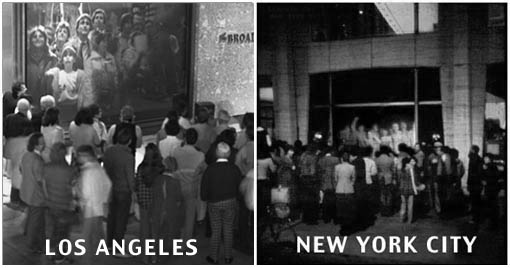
\includegraphics{figures/hole_in_space.jpg}
	\caption{Photos of the Hole in Space exhibit sites in Los Angeles and New York City.}
	\label{fig:hole-in-space}
\end{marginfigure}

\begin{marginfigure}
	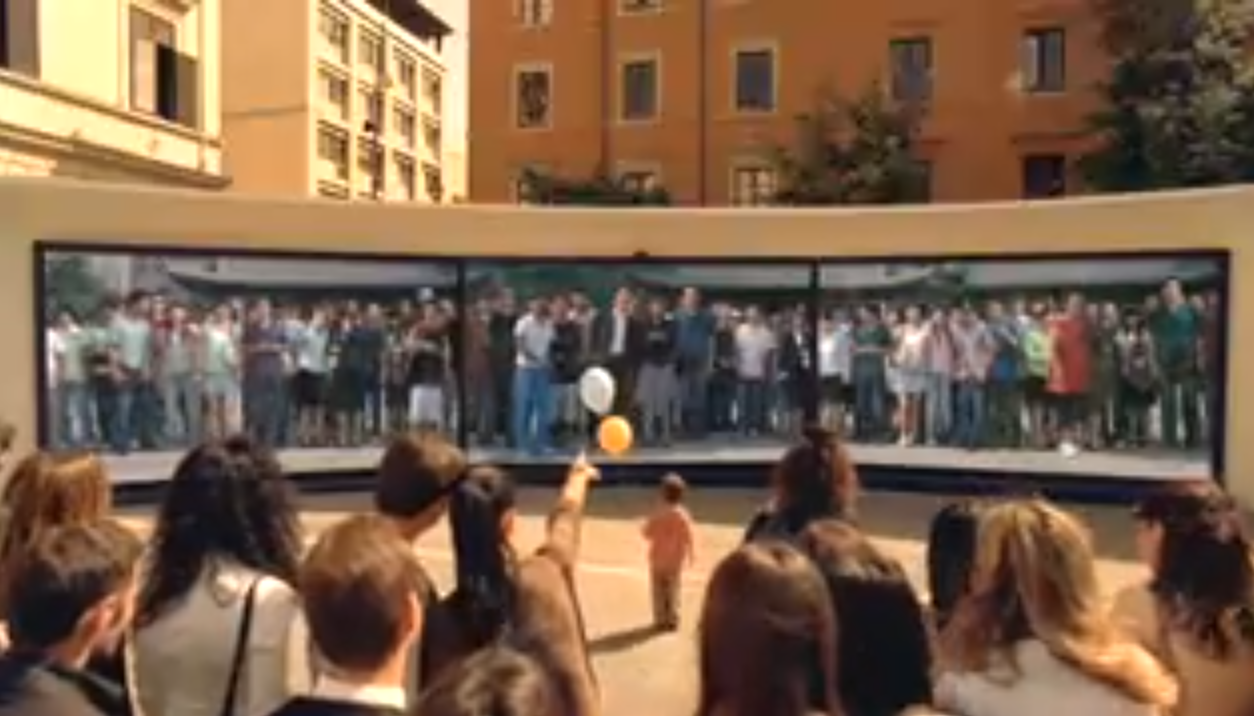
\includegraphics{figures/cisco-telepresence.png}
	\caption{Still from a Cisco Telepresence advertisement, centered on connecting an Italian piazza with a Chinese square with a seamless window.}
	\label{fig:cisco-telepresence}
\end{marginfigure}

% Despite these challenges, there's still an undeniable magic to the pursuit of recreating face-to-face communication at a distance. This magic is most poetically captured in the famous ``Hole in Space'' \citep{HoleinSpace:1980vn} piece, visually and audibly connecting a storefront in Los Angeles and New York in a way that seemed to make distance disappear. This vision is not simply aspirational, either. Tools to communicate with physically distant people either with audio alone or with an added video connection play a role in the daily lives of millions of people. This desire to experience ``being there'' with someone else is powerful and compelling.


\begin{marginfigure}
	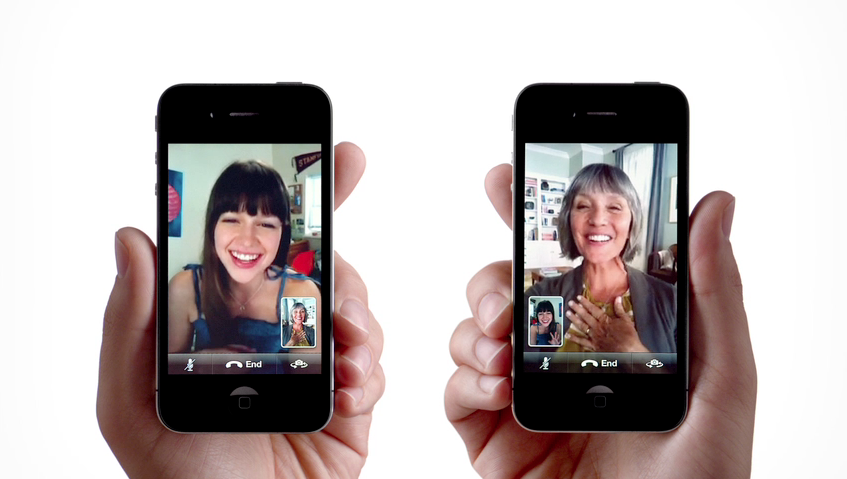
\includegraphics{figures/iphone-face-to-face.png}
	\caption{Still from an Apple advertisement demonstrating the Facetime feature to enable mobile video conferencing.}
	\label{fig:facetime}
\end{marginfigure}




\section{Complementary Communication}
This thesis addresses the design space of complementary communication systems. By this, I mean systems that aim to create a communication context shared by a group of people who are sharing some kind of experience like a presentation, performance, or discussion. Viewed this way, complementary communication systems are as old as whispering to someone sitting next to you or passing notes to a classmate. The addition of powerful personal communication technology to our everyday interactions have increased the opportunities we have to create complementary communication contexts as well as radically increased the reach a complementary communication system might have. In this context, how should we think about these sorts of systems? What goals should we have for them? In what contexts do they make sense? In particular, how should we think about the relationship between a complementary communication system in a face to face context? Is complementing a face to face interaction the same as complementing a mediated interaction?


In their famous paper, \citet{Hollan:1992tz} introduce the ``beyond being there'' approach. They argue that seeking to recreate the experience of ``being there'' was in a way an abdication of our responsibility as designers that left an important design space un-explored. In particular, they urge us to think less about ways to minimize the experience of mediation in communication, but to look instead for ways that mediation can add value to interactions. To take this perspective seriously, we need to shift away from a view of face-to-face interaction as being always better than interactions mediated by technology and instead think critically about potential limitations and challenges with face-to-face interaction and potential benefits that mediation can offer. 

\begin{marginfigure}
	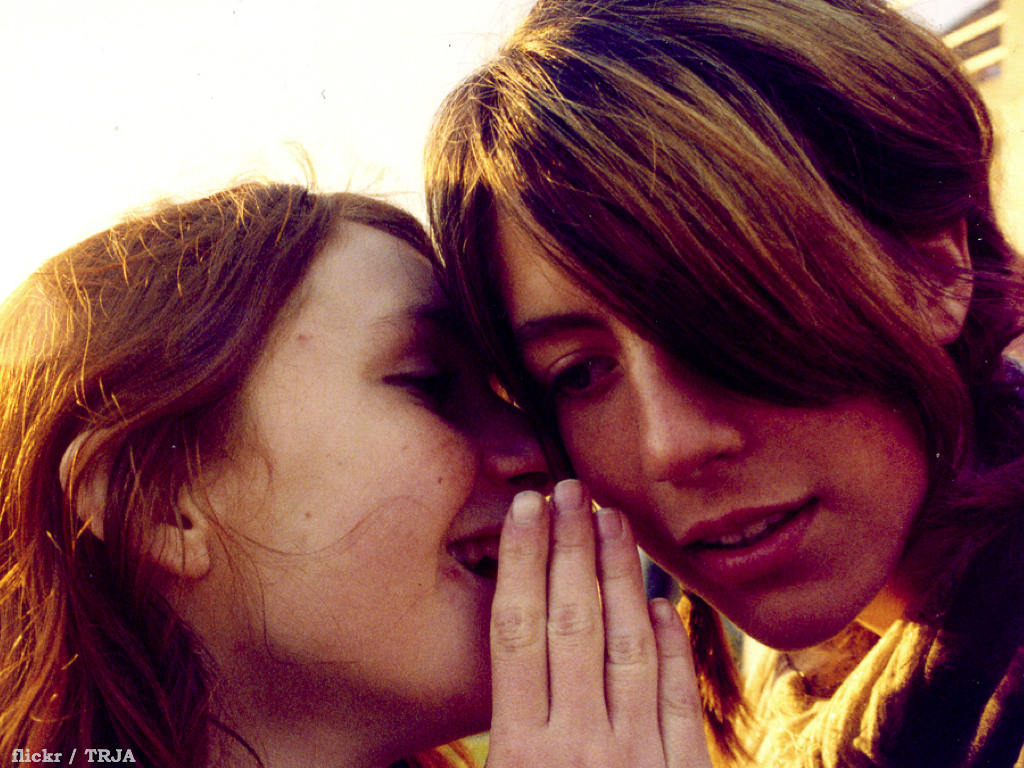
\includegraphics{figures/whisper.png}
	\caption{The original complementary communication experience.}
	\label{fig:whisper}
\end{marginfigure}


Although Hollan and Stornetta focus on creating mediated experiences that rival or surpass face-to-face experiences, in my work I show that we don't have to choose one approach or the other. If we accept the argument that being face to face is not \emph{a priori} the best experience, the strategy I employ is to add complementary communication platforms that can be used simultaneously with face-to-face communication or mediated platforms that mimic face to face interaction.


\begin{marginfigure}
	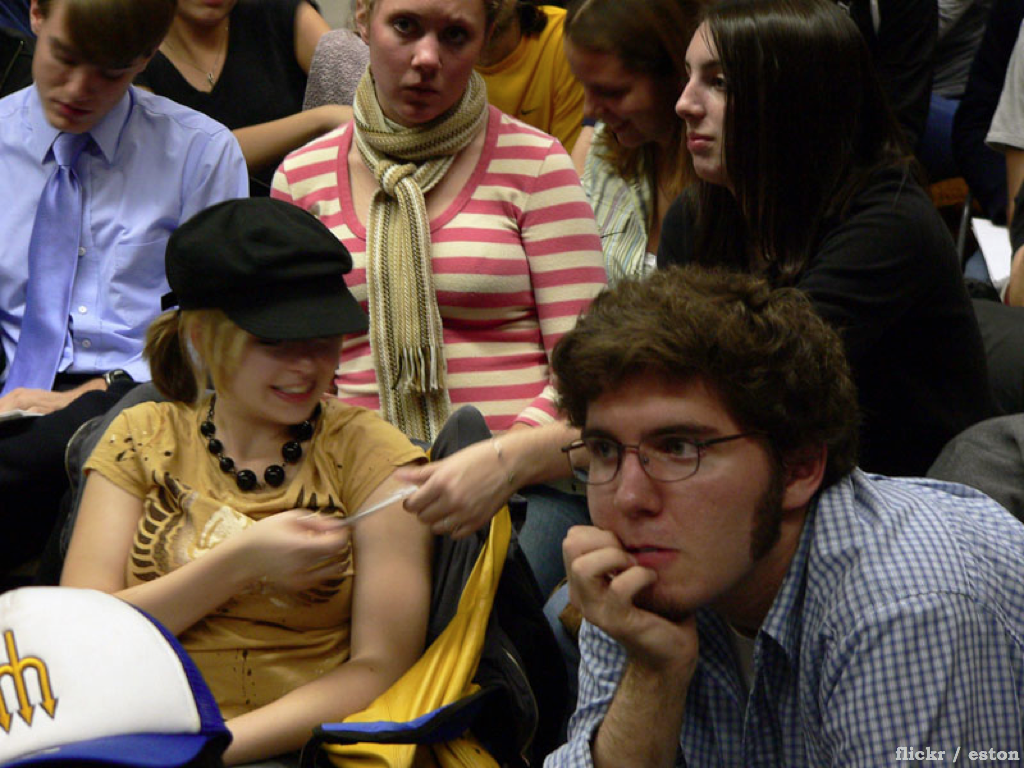
\includegraphics{figures/note-passing.png}
	\caption{The first complementary communication technology.}
	\label{fig:notes}
\end{marginfigure}


This easy equivalence between face-to-face communication and mediated imitations may seem unlikely; why should we accept that systems used in coordination with audio or video conferencing would be similar to those used to coordinate face-to-face? I will argue that a system that can effectively complement face-to-face interaction when its users could simply set it aside and rely on the (presumed superior) affordances of unfettered verbal communication likely has something to tell us about both design and face-to-face interaction more generally. If these systems can provide value in face-to-face contexts, I will show that they also provide value (perhaps even more value) when used to complement systems that seek to create experiences \emph{like} being face-to-face. Furthermore, true ``distributed'' situations are becoming less common. Heterogenous configurations where some people are co-located and others are remote and possibly alone are becoming more common. In these contexts, a system that doesn't operate effectively between co-located users is unlikely to be broadly useful, and would suffer from the disenfranchising effects we see for people who ``dial in'' to a local meeting. Thinking broadly about systems that complement both face-to-face and audio/video sharing will more efficiently lead us to systems effective in both contexts than treating them as separate cases.

\begin{marginfigure}
	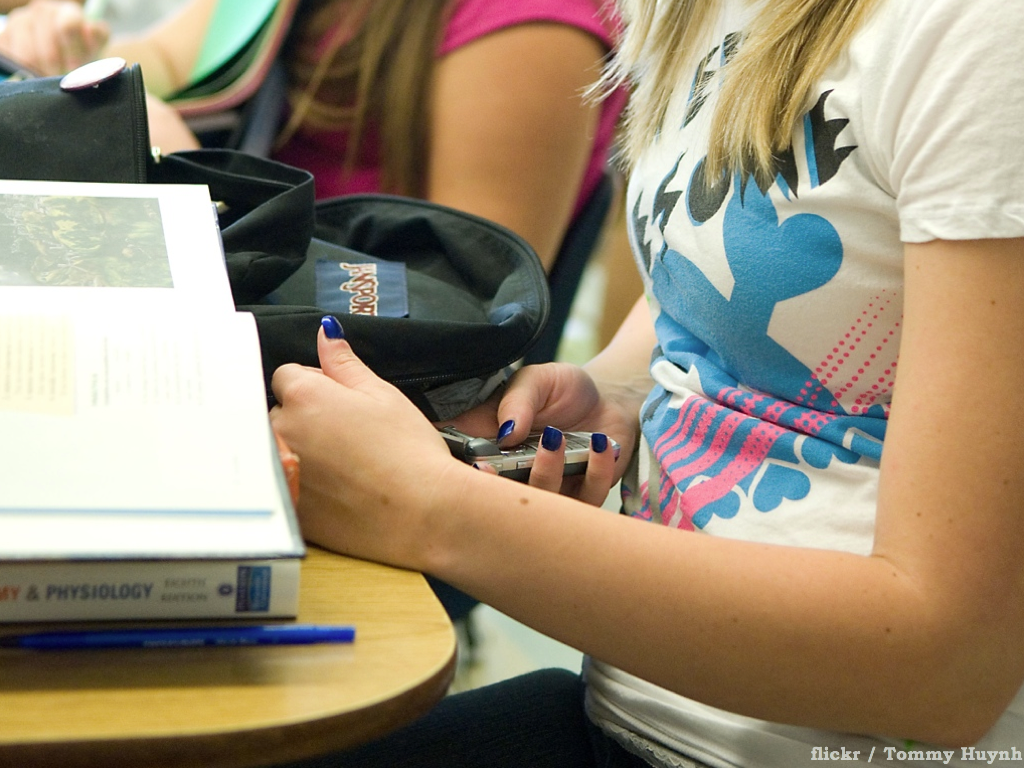
\includegraphics{figures/texting.png}
	\caption{Person to person text messaging extends the reach of something like note passing to include anyone with a phone. Phones also support multi-party conversations, increasing the size of the audience for complementary communication systems.}
	\label{fig:texting}
\end{marginfigure}




% think about listifying this section

% Many of these challenges are common sense, even if they are frequently forgotten when people argue for recreating face-to-face experiences. Face-to-face communication requires relatively explicit turn-taking; multiple speakers in a group make them all largely unintelligible. In mediated environments like chat, simultaneous conversation threads can easily co-exist for long periods of time. There are major identity implications to face-to-face communication. It is difficult to conduct any face-to-face communication without revealing significant information about your identity. In mediated contexts, there are techniques ranging from anonymity to pseudonymity to limit identity disclosing information. Participation in non-mediated interactions is ephemeral, while mediated interaction can easily be archived and represented either in context or after the fact. Participation in face-to-face situations can be limited by confidence, but mediated participation tends to be more disinhibited. \citep{Siegel:1986ve}

% is this a second order effect?
% For a variety of reasons, the power dynamics in social situations are more easily subverted in mediated environments. 

This dissertation is organized around a series of ``primary'' contexts for which I design a particular complementary communication system that enhances the overall experience. Metrics and evaluation strategies vary for each of these pieces, but each project shares a deep interest in trying to fill in the gaps of the ``primary'' interaction space by using the particular strengths of some additional mediated communication system. The goal of these interventions is to create environments where people have ways to express themselves non-verbally in addition to whatever existing communication channels exist, often audio, sometimes visual. By adding mediated communication channels to other existing channels, we can focus each channel on its primary affordances and let it do what it does best while letting the complementary communication channels fill in the gaps.


\section{From Channel To Stage}

Platforms for discussion and commenting that are outside official discourse channels have widely been referred to as ``backchannels.''  Backchannels, traditionally defined, create a space where audience members to some ``front channel'' can share information with each other, typically about the content of the front channel. \sidenote{This is in contrast with the traditional technical use of ``backchannel'', which refers to the verbal and non-verbal cues that non-speaker give a speaker during a conversation. In this usage, backchannel was a type of communication, not an actual dedicated distinct channel the way it is in this context.} This metaphor is an apt description of much of the prior work in this space, like \citep{Cogdill:2001fp,Yardi:2006uk,mccarthy_digital_2004,Rekimoto:1998jy}. I have found, however, that it is not as useful for understanding the systems I will present in this thesis. Instead of using channels, I will argue for ``stages,'' and instead of a front/back separation, I will shift to a main/side distinction. \sidenote{Parts of the section to follow are adapted from \citep{Harry:2012df}.}


In a traditional backchannel configuration, audience members can view the front channel and have a variety of backchannels available to them, each with different sized audiences and affordances. This is represented in Figure \ref{fig:front-back-channel}. Presenters, on the other hand, often have a very hard time staying aware of backchannel content if they are aware of it at all. This asymmetry gives the backchannel its outsider flavor and can lead to disrespectful and unproductive content \citep{boyd:Yo36SNyj}. This is widely recognized as a major problem with backchannels. In this way, the front/back distinction is an accurate description of existing systems, but not a situation I seek to recreate. \sidenote{Of course, there may be contexts where the front/back distinction is valuable. But since that is the predominant structure for existing tools, there are many more options for supporting that approach so I don't give it much attention in this thesis.} Mitigating this sense of separation is a major design goal in my work.





% In this configuration, the front/back channel distinction is a useful one because in a very practical sense the backchannel is usually somewhat covert or hidden and participants in the backchannel rarely have the ability or opportunity to communicate on the front channel. \sidenote{This paragraph and the rest of this section are largely from \citep{Harry:2012df}.} 

% I wonder if it's worth putting some examples here? I thiiink we can get away without, but might help ground people's thinking.

% Although this front/back channel metaphor works in situations where audience members have no access to the front channel, it is less effective in situations where the backchannel is intended to influence the front channel. 

% As will be discussed in the related work, much recent work is focused on bridging these front and back spaces and I argue through the work presented in this thesis that a new metaphor is useful for understanding how these parallel communication spaces can be configured.

To enable this shift, we need to re-imagine the nature of social interaction in these sorts of spaces. A channel metaphor implies a clear split between those empowered to broadcast, and an audience who receives that broadcast. It also has implications for how attention is managed; channels imply a model of binary attention. To find an alternative, I turn to \citet{goffman_presentation_1959} for his description of \emph{stages} to illuminate this new sort of situation. He uses the example of a waiter behaving politely with a problematic customer and then walking into the kitchen and complaining to the cook about the customer's difficult behavior. Each interaction is performative and represents the waiters' competence at performing his role appropriately for different audiences in a different setting. In the waiter example, these audiences are disjointed, and the door into the kitchen represents a gateway between the ``front'' performance space with customers and the ``back'' performance space among restaurant staff. The notion of stages shifts our attention from spaces where a small number of people can broadcast information to many recipients (like a lecture hall or conference) and instead focuses on negotiated sites of performance like the restaurant dining room and kitchen, where people can perform different aspects of their identity for different audiences. This intermediate state is shown in Figure \ref{fig:front-back-stage}. In this model, the back stage still lacks accessibility for much of the audience, and is not easily perceived by performers on the front stage.

\begin{marginfigure}
	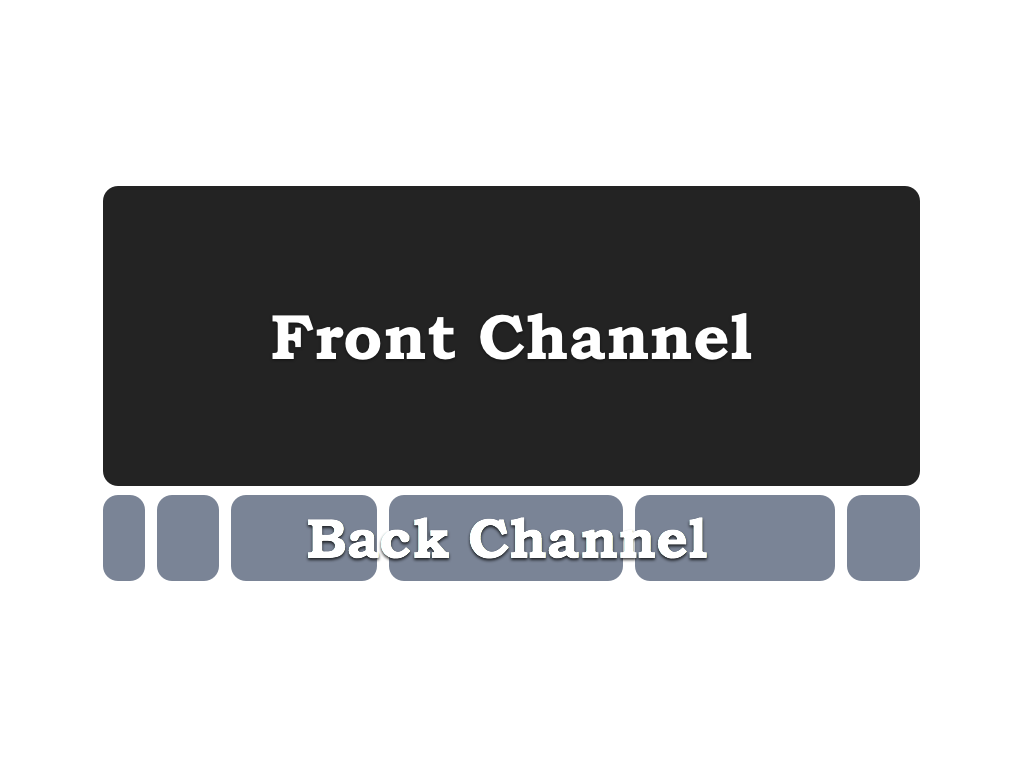
\includegraphics{figures/front-back-channel.png}
	\caption{The conceptual model inherent in a front/back channel configuration.}
	\label{fig:front-back-channel}
\end{marginfigure}

\begin{marginfigure}
	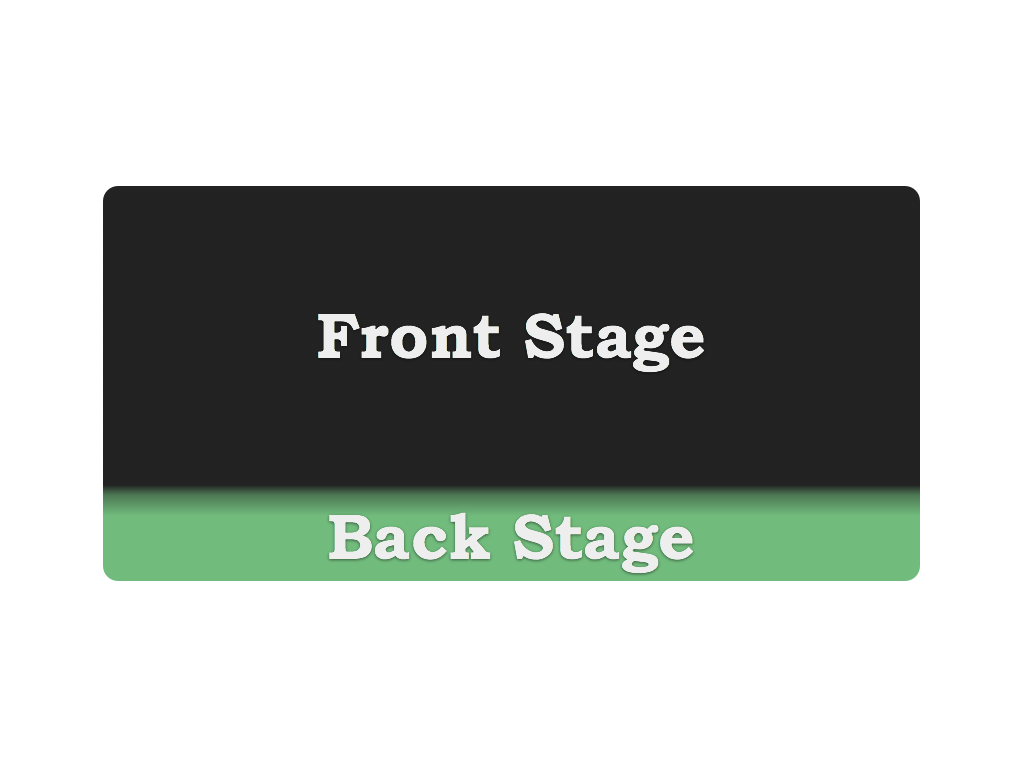
\includegraphics{figures/front-stage-back-stage.png}
	\caption{The transition from channels to stages; brings the audience closer to the performer and increases the visibility of the back stage.}
	\label{fig:front-back-stage}
\end{marginfigure}

This notion of stages is a useful metaphor to replace channels. Unlike channels, where audiences are basically invisible to the performer, stages bring the audience and performer together and create a context in which they are mutually aware of each other. Stages also shift from the notion of a small group of broadcasters and a large group of receivers, to a context where there is the potential for different performers at different moments. The notion of stages also more actively recognizes the way that audiences to a performance are themselves constantly performing in small ways, while a channel metaphor limits the audience to simply receiving a broadcast. This comprises both small performances and the potential for substantial performances. In a large lecture hall, the nature of the individual performance is not that precise. If there is an open laptop policy, audience members might be checking their email or engaging in an official backchannel.  They are able to, as Goffman says, ``get away with going away," because the act of \emph{going away} is an expected part of being in the audience to a front stage performance. But a shift from channels to stages is important in recognizing that even as audience members, looking at a laptop screen instead of the teacher is a sort of small performance. Furthermore, a student may raise their hand and ask a question of the teacher, thus assuming a larger role in the main stage.

\begin{marginfigure}
	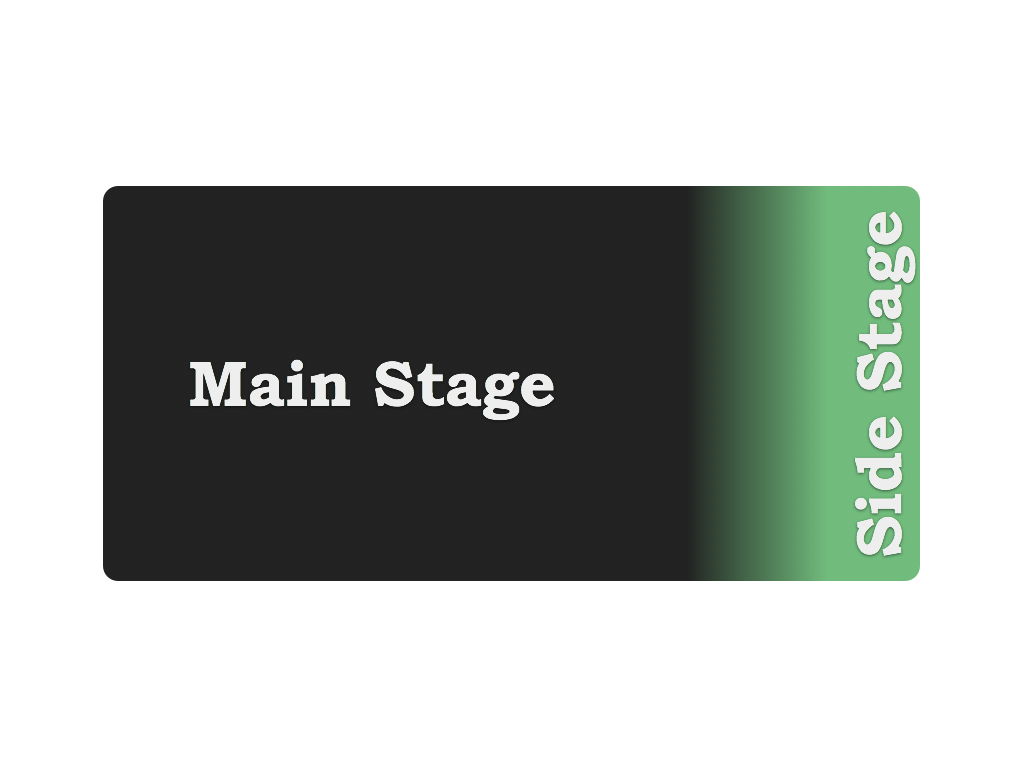
\includegraphics{figures/main-side-final.png}
	\caption{The final conceptual model that I argue for. Main and side stage are well blended and can influence each other. Main stage and side stage share an audience.}
	\label{fig:main-side-stage}
\end{marginfigure}


Although Goffman's description of appropriate performances for a specific audience is valuable, we want to avoid that front-back distinction as enacted in his restaurant example. Instead of having separate audiences, we want to create a space where, although the modes of performance are different, the performances are available to everyone. While in a channel metaphor, audiences are split between multiple back channels which are largely unavailable to someone performing on the front channel, stages create the opportunity for situations where the audiences for each stage can be shared. This unified audience helps us move away from the front/back distinction to a main/side distinction. In this model, performances on the main or side stage both share one large audience. By unifying the audiences, we can help avoid the problem with backchannels where they tend to assume a covert character. If side stage participation is accessible to everyone, it changes the character of the communication. Side stage performances lose some of their covert nature because they can be seen by a larger audience that includes main stage performers. Simultaneously, main stage performers can be made actively aware of side stage performances in a way that is inclusive, to help them better react to their now more present audience.

To reiterate, this change in metaphor has two components: a shift from channels to stages, and a shift from front/back to main/side. This is an aspirational shift; most of the design work in this space to date has represented the backchannel approach. But if these systems are to be an effective addition to face-to-face-type experiences, I will show how adopting this new metaphor can create effective communication experiences that encompass multiple simultaneous opportunities for engagement that create an effective, unified experience. This final configuration is shown in Figure \ref{fig:main-side-stage}. 


In my initial argument against the sufficiency of un-augmented face-to-face communication, I aimed to show how moving from a single stage to a main and side stage can be valuable, provided the side stage is designed to complement the potential deficiencies of the main stage. It is not obvious that a single side stage is the only effective configuration. Why is one side stage the appropriate number? Why might we not prefer a multiplicity of side stage, with audience attention shifting fluidly between them? Intellectually, a model that supports a network of stages with various properties and interactions is, as in actor network theory \citep{latour_reassembling_2007}, seems attractive. Stopping at two stages seems to make the same mistake of enshrining a particular form of interaction as optimal, and leave the model open to the same argument I make against main-stage-only experiences.

Although describing such a network-based theory is not the focus of this thesis, I would definitely view it as an effective tool for understanding interactions in existing backchannel-based ecosystems. Backchannels are rarely monolithic and in most situations a large number of backchannels are operating simultaneously. Most are out of sight for non-participants (like instant messaging and chat), while some strive for ``official'' status (like \emph{Twitter}) and can start to feel more like a single monolithic backchannel. Thus while a model that supports a multitude of simultaneous complementary communication systems is an accurate picture of most experiences, it is not necessarily a model we want to be encouraging from a user experience perspective. As discussed in the transition from a front/back to main/side configuration, attempting to unify the audiences between the front and back stages represents one of our major tools to mitigate the covert effects of backchannels with distinct, separate audiences. Without blessing a particular stage as ``the'' side stage, we would run the risk of creating just another backchannel with the challenges to driving adoption, creating integration with the main stage, and covert flavor that I identify in contexts with a variety of backchannel options.

Realistically, we are always embedded in networks of communication contexts that include both people we are physically co-located with and remote people. These overlapping networks of text messaging, \emph{Facebook} updates, and tweets are part of our professional and personal lives most of the time. Even in a context with a single designated side stage, it would be unreasonable to expect that there aren't also a variety of backchannels operating simultaneously. Complementary communication systems must compete effectively with these backchannels to provide a meaningful space for interaction if they hope to succeed, and it would be na\"{\i}ve to ignore them from a design perspective. We could extend the main stage/side stage model to make room for multiple overlapping side stages, but we run a practical risk of overwhelming an audience or group, and turning each of the side stages into distinct backchannels that fail to command a unified audience or influence the main stage in a productive way. Because of these practical challenges, I set aside the problem of modeling stages in a more elaborate network context and focus instead on single side stages paired with a main stage, and seek to understand that relationship from theoretical and practical perspectives.

% overall points to make here
% 	- don't want to enshrine 


% Each is a performance, but the backstage is presumably more authentic. So unlike the concept of channels, which are composed of discreet information streams, stages are negotiated sites of performance around a singular situation.

% Instead of the metaphor of channel, he would refer to these alternate communication streams as stages.  When one moves from formal interactions to less formal interactions, one moves from front to back stage. When on the front stage, performance is prescribed and specific roles can be rigid.  And when on the back stage, one is more free to authentically represent themselves and their thoughts about the front stage.  He uses the example of a waiter behaving one way with a customer and then walking into the kitchen and telling the cook about the customer's difficult behavior.  Each is a performance, but the backstage is presumably more authentic. So unlike the concept of channels, which are composed of discreet information streams, stages are negotiated sites of performance around a singular situation. 






% This shift from 
% 
% 
%  But in a seminar environment, attentiveness and participation are more scrutinized because of the size and nature of the group. This suggests that integrating new communication technology into groups of smaller size might be more challenging because \emph{going away} is more difficult to politely incorporate into the front stage performance.  
% 
% 
% Communication systems used in a context where they are not the primary communication channel have historically been referred to as ``backchannel'' communication systems. Chat-oriented systems were the most popular, and have been deployed in a variety of contexts, though research has often focused on  conferences \citep{mccarthy_digital_2004, Rekimoto:1998jy} and classrooms \citep{Cogdill:2001fp,Yardi:2006uk} as fertile spaces for these sorts of interventions. More recently, tools like \emph{Twitter} have been described as a ``backchannel'' for live events. In some cases, a live-updating feed of recent tweets containing certain event-specific keywords have been projected in the space.
% 
% Although my work seems at first glance to fall into this same category of backchannel designs, I argue that a shift in the categories we use to think about these systems is important for building effective spaces. 
% 
% 
% 
% 
% In the literature about mediated communication systems used in a context where they are not the primary channel

 % Need to introduce stages as a concept here! Do the whole backchannel -> side stage transition argument here? It has to happen somewhere and it has to happen EARLY. It doesn't happen anywhere in background yet. 


\section{Design Spaces, Themes, and Theory}

One of the challenges of building technical systems as research is understanding the scope of conclusions. If you took a particular design element into a different system, would it operate in the same way? What are the relationships between the sorts of people using the system and the socio-technical structures that emerged? These are difficult questions to answer within the scope of a single project. The researcher may have solid intuition, but the tendency of the researcher is probably to see overly-general results more often than overly-specific results. One of the ways I address this is by describing a series of projects in this design space and examining design elements and themes in a variety of contexts.

This would be less effective as an approach if each of the design spaces was quite similar. The contexts I am designing for can be organized around a series of major differentiating axes:

\begin{description}
\item[Main Stage]{The medium for the main stage, e.g. the site of the primary shared experience of the audience.}
\item[Shared Display]{The presence or absence of a shared display.}
\item[Side Stage Attention]{The frequency of audience attention on the side stage. This is quite qualitative and varies across users, but each system embeds contains certain assumptions about the relative importance of the side stage to the main stage.}
\item[Audience Size]{The target audience size for the system.}
\end{description}

Table \ref{tab:project-axes} lists the research contexts covered in this dissertation, and describes each project's location on the major context axes. The variety across these axes helps show the breadth and scope of my work. 
\begin{table*}[tb]
	% \centering

\begin{tabular}{r|llll}
& Main Stage & Shared Display & Side Stage Attention & Audience Size \\
\hline
\textbf{backchan.nl} & face-to-face & yes & infrequent & 20-500 \\
Information Spaces & virtual world & yes & infrequent & 10-20 \\
ROAR & broadcast video & no & frequent & > 1,000 \\
\textbf{Tin Can} & face-to-face & no & occasional & 10-20 \\
\end{tabular}
\label{tab:project-axes}
\caption[][15pt]{Comparing the projects covered in this dissertation on the major axes that distinguish them. Projects in bold are major projects discussed in the most depth. Small project variants (e.g. backchan.nl for remote Q\&A, Tin Can Meetings, etc.) are not included.}
\end{table*}

% could I identify a set of common design elements that can be traced across all projects?
% voting
% chat
% shared display?

Although each project operates in a different context, there are a number of research themes that each project addresses. Although these themes were not identified at the start of this research stream, they nonetheless are present in all my work to various degrees. It can be challenging to identify the broader impact of design-based research (a topic I will address in more depth in the next chapter), but it is through looking at these themes in different contexts that I hope to contribute to broader discussions. These are themes that are relevant particularly to designing complementary interfaces like those in my own work, but also to many kinds of collaborative, synchronous systems, even those which aren't trying to create complementary experiences.

\begin{description}
	\item[Grounding]{My work uses shared displays in a variety of different capacities. I contend that these kinds of public displays can play a powerful role in helping to ground, in the \citet{Clark:1989uc} sense, a conversation. In particular, shared displays can provide ways to non-verbally acknowledge discourse presentations. By their very shared nature, the contents of shared displays might accelerate the creation of common ground. The different ways that these shared displays operate in my work helps provide insight into both particular design techniques to support grounding as well as the broader discussion around how common ground operates in mediated communication contexts.}
	\item[Non-verbal actions]{As a result of the drive to create a sense of ``being there'', mediated interaction systems failed to consider the ways that we communicate non-verbally, assuming that higher fidelity video and audio would be sufficient to capture that communication. I contend that our non-verbal actions in the physical world are a critical component of body language, and when creating mediated channels we should strive to create new vocabularies of action that enable people to communicate non-verbally. In much the same way that in a shared physical space we can observe people interact with objects around us, so too should people's actions in mediated systems be visible and part of supporting a sense of presence and awareness. How these action vocabularies are constructed and communicated to people is critical to the success of these sorts of systems.}
	\item[Attention]{Creating new opportunities for simultaneous commentary and communication about some shared experiences creates situations where people have to make choices about which if the stages to attend to and which stage to use for their performances. From a design perspective, there are a number of important attention related decisions to make: How is our attention made visible to others, and how does it affect their impressions of us? How do we design displays for occasional attention of users who are shifting their attention between different stages? Understanding how people think about and enact attention in situations with multiple available communication channels is critical to designing appropriate options and understanding the practices that evolve around them.}
\end{description}

This work contributes on two levels. First, by creating and deploying interfaces with particular properties, I provide concrete guidance and insight about particular specific design strategies and interfaces. This is valuable for designers and researchers thinking about how they design this variety of communication systems. I also contribute to the broader discourse about the three research themes laid out above. In each case there are both broader theoretical contributions to be made as well as specific findings that contribute to scholarly discussions about these issues.

\section{Thesis Organization}

This thesis starts with a broad background discussion about some of the methodological assumptions implicit in doing design work as research, a tour through some of the high level related work that all of my work relies on, and a more in-depth treatment of the major research themes I introduced here.

Based on this background, I will then discuss four major project areas in each of the following four chapters: Virtual Worlds (which contains two specific sub-projects for meetings and presentations in virtual worlds), \emph{backchan.nl} (a tool for managing audience feedback during live events), \emph{Tin Can} (a tablet-based platform for enhancing small group discussions), and \emph{ROAR} (a platform for very large scale audience interaction during live events). Through each of these chapters I will relate my findings back to the research themes that are laid out in Chapter \ref{ch:background}. 